\documentclass{article}

\usepackage{graphicx}
\usepackage{amsmath}
\usepackage{fancyhdr}
\usepackage[sorting=none]{biblatex}
\usepackage[margin=1in]{geometry}
\usepackage[font={small,it}]{caption}
\usepackage{placeins}
\usepackage{xepersian}

%\DeclareMathOperator*{\btie}{\bowtie}
\addbibresource{bibliography.bib}
\settextfont[Scale=1.2]{B-NAZANIN.TTF}
\setlatintextfont[Scale=1]{Times New Roman}
\renewcommand{\baselinestretch}{1.5}
\pagestyle{fancy}
\fancyhf{}
\rhead{تکلیف اول درس پایگاه داده‌ها 1}
\lhead{\thepage}
\rfoot{علیرضا ابره فروش}
\lfoot{9816603}
\renewcommand{\headrulewidth}{1pt}
\renewcommand{\footrulewidth}{1pt}

\begin{document}
\begin{titlepage}
\begin{center}

\includegraphics[width=0.4\textwidth]{figures/IUT Logo.png}\\
        
\LARGE
\textbf{دانشگاه صنعتی اصفهان}\\
\textbf{دانشکده مهندسی برق و کامپیوتر}\\
        
\vfill
        
\huge
\textbf{عنوان: تکلیف چهارم درس ریزپردازنده}\\
        
\vfill
        
\LARGE
\textbf{نام و نام خانوادگی: علیرضا ابره فروش}\\
\textbf{شماره دانشجویی: 9816603}\\
\textbf{نیم\,سال تحصیلی: پاییز 1400}\\
\textbf{مدرّس: دکتر عارف کریمی افشار}\\
\end{center}
\end{titlepage}


%\tableofcontents
\newpage

\section{}
اگر سوال بخش\,بندی\,شده نباشد، پاسخ آن در این قسمت نوشته می\,شود.
\subsection{}
\begin{itemize}
    \item [$\bullet$]
    \lr{DBMS}
    به عنوان واسطه بین کاربر و پایگاه داده عمل می‌کند. این ساختار پایگاه داده خود به عنوان مجموعه ای از فایل‌ها ذخیره می‌شود و تنها راه دسترسی به اطلاعات موجود در آن فایل‌ها از طریق 
    \lr{DBMS}
است.
شکل 1.1 بر این نکته تأکید می کند که
    \lr{DBMS}
به کاربر (یا برنامه کاربردی) یک نمای واحد و یکپارچه از داده‌های موجود در پایگاه داده ارائه می دهد.
    \lr{DBMS}
همه 
	\lr{request}
‌های برنامه را دریافت و آن‌ها را به عملیات‌های پیچیده مورد نیاز برای پاسخ به 
این
	\lr{request}
‌ها
ترجمه می‌کند.
بسیاری از پیچیدگی‌های داخلی پایگاه داده به وسیله 
    \lr{DBMS}
از برنامه های کاربردی و کاربران پنهان می‌شود.
برنامه کاربردی ممکن است توسط یک برنامه‌نویس با استفاده از یک زبان برنامه‌نویسی مانند 
	\lr{Visual Basic.NET}، \lr{Java}
یا
	\lr{C\#}
نوشته شود یا ممکن است توسط یک
	\lr{DBMS utility program}
ساخته شود.
داشتن یک
	\lr{DBMS}
بین
	\lr{application}
کاربر و پایگاه داده مزایای مهمی را به ارمغان می‌آورد. اولا
	\lr{DBMS}
به داده‌ها اجازه می‌دهد که بتوانند بین چندین برنامه به اشتراک گذاشته شوند. ثانیا
	\lr{DBMS}
بسیاری از دیدگاه(\lr{view})های مختلف کاربران از داده‌ها را با هم ادغام می‌کند و در یک مخزن همه جانبه ارائه می‌دهد.
\begin{figure}[ht]
    \centering
    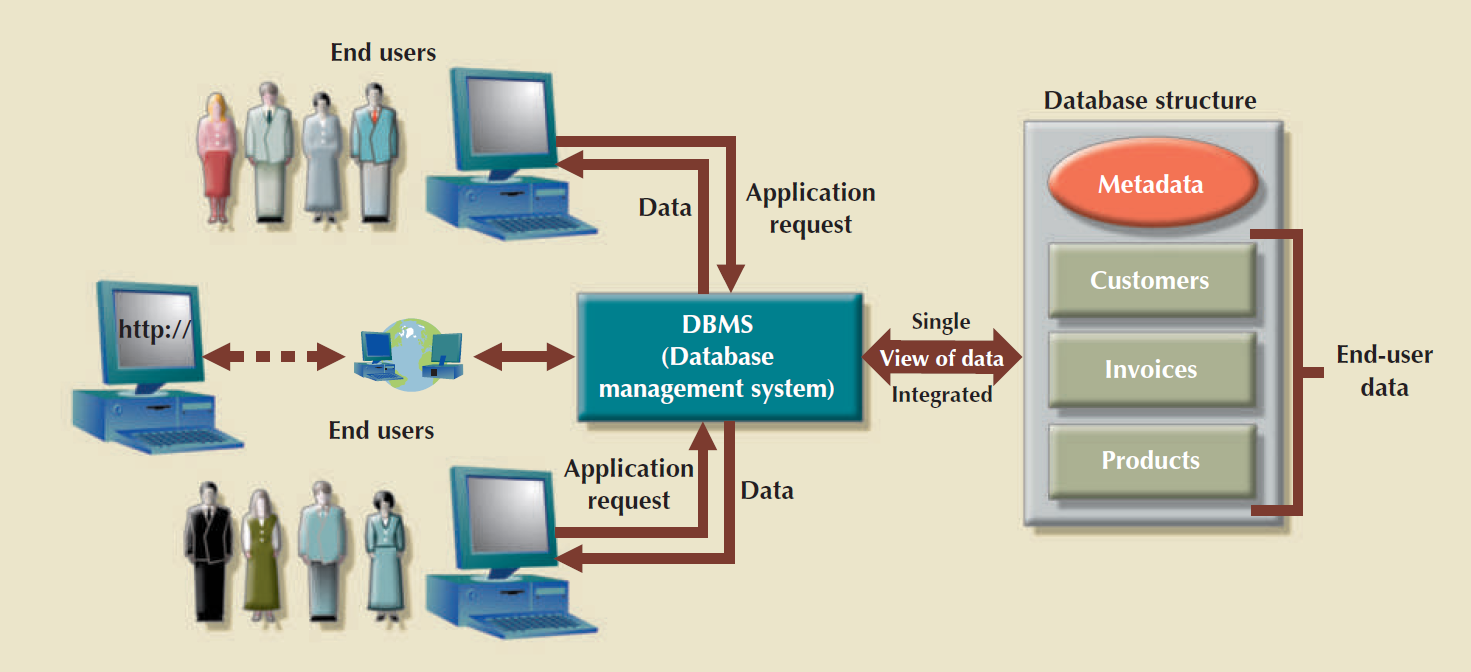
\includegraphics[width=0.7\textwidth]{figures/1.1.png}
    \caption
	{
	\lr{DBMS}
تعاملات بین کاربر و پایگاه داده را مدیریت می‌کند.
	}
    \label{fig:fig1}
\end{figure}

%%%%%%%%%%%%%%%%%%%%%%%%%%%%%%%%%%%%%%%%%%%%%%%%%%%%%%%%%%%%%%%%%%%%%%%%%%%%%%%%%%%%%%%%%%%%%%%%%%%%%%%%%%%%%%%%

%%%%%%%%%%%%%%%%%%%%%%%%%%%%%%%%%%%%%%%%%%%%%%%%%%%%%%%%%%%%%%%%%%%%%%%%%%%%%%%%%%%%%%%%%%%%%%%%%%%%%%%%%%%%%%%%
    \item [$\bullet$]
افزونگی داده‌ها و ناسازگاری(داده ها در چندین فرمت فایل ذخیره می شوند و در نتیجه افزونگی کمتری از اطلاعات در فایل های مختلف رخ می‌دهد)، سخت بودن دسترسی به داده‌ها(نیاز به نوشتن یک برنامه جدید برای مدیریت هر تسک جدید)، ایزولگی داده‌ها، مشکلات یکپارچگی،آپدیت اتمیک ، دسترسی همزمان توسط چند کاربر، مشکلات امنیتی
\end{itemize}
\subsection{}
گام‌های طی شده توسط
\lr{DBMS}
جهت پاسخ به درخواست کاربر(\lr{query}) در شکل 2 مشخص شده است.
گام‌های پایه عبارتند از:
\newline
\begin{enumerate}
    \item
پارس و ترجمه(\lr{Parsing and translation})
    \item
بهینه‌سازی(\lr{Optimization})
	\item
ارزیابی(\lr{Evaluation})
\end{enumerate}
پیش از اینکه
\lr{query processing}
آغاز شود، سیستم باید
\lr{query}
را به یک فرمت قابل ترجمه تبدیل کند. یک زبان مانند
\lr{SQL}
برای این کار مناسب می‌باشد، اما همچنان جهت نمایش داخلی
\lr{query}
در یک سیستم مناسب نیست. یک راه مبتنی بر جبر رابطه ای وجود دارد که مناسب‌تر است.
\newline
ابتدا سیستم درخواست را به یک
\lr{query}
تبدیل می‌کند. از اینجا به بعد پردازش بر عهده
\lr{DBMS}
است که
\lr{query}
را به عبارتی تحت عنوان جبر رابطه‌ای پارس و ترجمه(این ترجمه شبیه به کاری است که پارسر کامپایلر انجام می‌دهد) می‌کند و سپس بهینه(چند روش ممکن) می‌کند و در انتخاب روش به آمار و سایز جداول توجه می‌کند. حال
\lr{DBMS}
به یک
\lr{execution plan}
رسیده است که چگونگی اجرای دستور وارد شده توسط کاربر را نشان می‌دهد. سپس در اختیار
\lr{evaluation engine}
قرار می‌گیرد که در این گام به سراغ داده‌ها می‌رود و آن‌ها را کنار هم می‌چیند و خروجی را برمی‌گرداند.

\begin{figure}[ht]
    \centering
    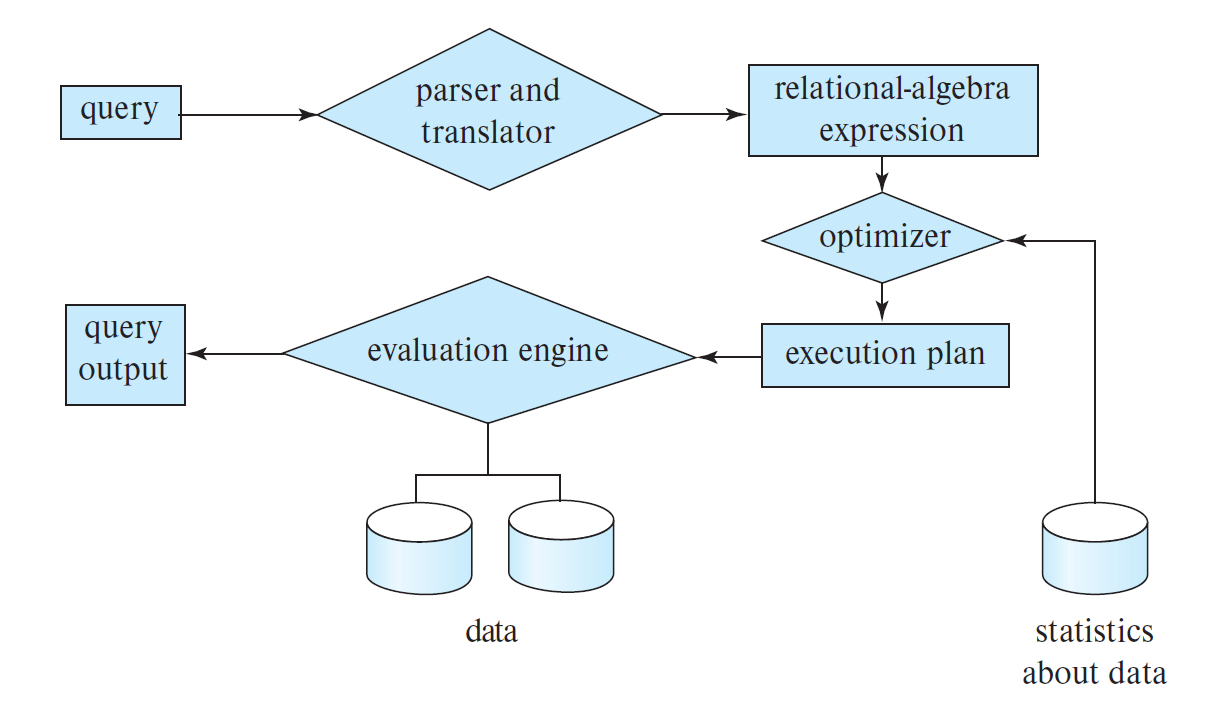
\includegraphics[width=0.8\textwidth]{figures/1.2.png}
    \caption
	{
گام‌های پردازش
\lr{query}
	}
    \label{fig:fig1}
\end{figure}
\FloatBarrier

\subsection{}
پاسخ بخش سوم سوال در این قسمت نوشته می\,شود.
\begin{figure}[ht]
    \centering
    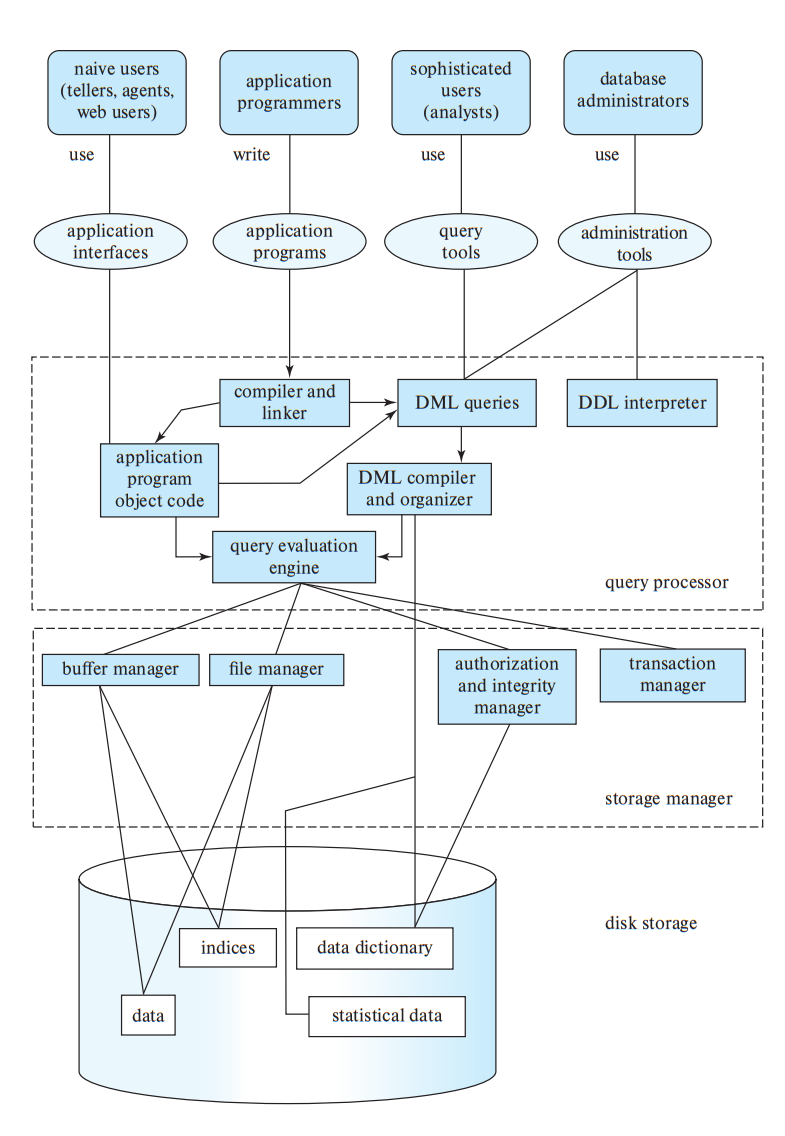
\includegraphics[width=0.8\textwidth]{figures/1.3.png}
    \caption{}
    \label{fig:fig1}
\end{figure}
\FloatBarrier

\section{}
ابجدهوز
\begin{figure}[ht]
    \centering
    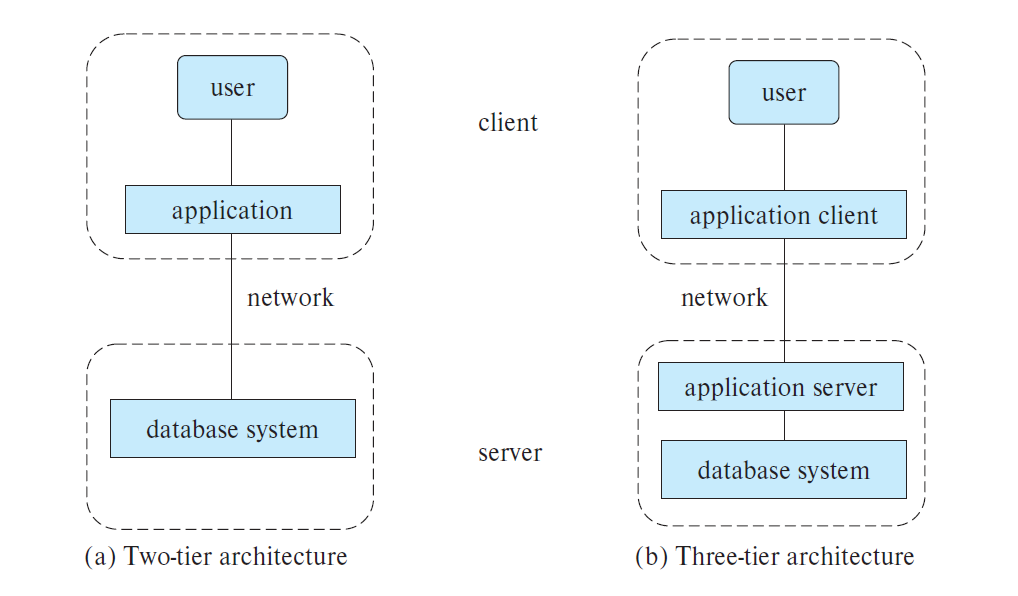
\includegraphics[width=0.8\textwidth]{figures/2.png}
    \caption{}
    \label{fig:fig1}
\end{figure}
\FloatBarrier
\begin{table}[ht]
    \centering
    \begin{tabular}{|c|c|c|}
    \hline
    ویژگی‌ها & معماری دولایه & معماری سه‌لایه\\
    \hline
    سرعت & کمتر(کندتر) & بیشتر(سریعتر)\\
    \hline
    امنیت & کمتر(کلاینت می‌تواند مستقیما با پایگاه داده تعامل داشته باشد) & بیشتر(کلاینت مجاز به تعامل مستقیم با پایگاه داده نمی‌باشد)\\
    \hline
    افزونگی & خانه شماره 5 & خانه شماره 6\\
    \hline
    مقیاس‌پذیری & کمتر() & بیشتر()\\
    \hline
    انعطاف‌پذیری & خانه شماره 5 & خانه شماره 6\\
    \hline
    یک‌پارچگی & خانه شماره 8 & خانه شماره 9\\
    \hline
    \end{tabular}
    \caption{جدول شماره 1}
    \label{tab:tab1}
\end{table}

\section{}
اگر سوال بخش\,بندی\,شده نباشد، پاسخ آن در این قسمت نوشته می\,شود.
\subsection{}
پاسخ بخش اول سوال در این قسمت نوشته می\,شود.
\subsection{}
پاسخ بخش دوم سوال در این قسمت نوشته می\,شود.

\section{}
اگر سوال بخش\,بندی\,شده نباشد، پاسخ آن در این قسمت نوشته می\,شود.
\subsection{}
پاسخ بخش اول سوال در این قسمت نوشته می\,شود.
\subsection{}
پاسخ بخش دوم سوال در این قسمت نوشته می\,شود.
\subsection{}
پاسخ بخش دوم سوال در این قسمت نوشته می\,شود.
\subsection{}
پاسخ بخش دوم سوال در این قسمت نوشته می\,شود.

\section{}
\subsection{}
$
\Pi_{Title,\:ReturnDate}
(Borrow \bowtie_{MemberID\:=\:1356\:\wedge\:IsReturned\:=\:false} Book)
$

\subsection{}
$
\Pi_{Name}
(Member
\bowtie_{Member.CategoryID\:=\:``Physics"}
(Book \bowtie_{Book.BookID\:=\:Borrow.BookID\:\wedge\:CategoryID\:=\:``Physics"}\:Borrow))
$
\subsection{}
$
\Pi_{Name,\:Title}
(Member
\bowtie_{Member.CategoryID\:=\:Book.CategoryID}
Book)
\:-\:
\newline
\Pi_{Name,\:Title}
(Borrow
\bowtie_{Borrow.MemberID\:=\:Member.MemberID\:\wedge\:Borrow.BookID\:=\:Book.BookID}
\newline
(Member
\bowtie_{Member.CategoryID\:=\:Book.CategoryID}
Book))
$
\subsection{}
$
\Pi_{Name,\:Title}
(Member
\bowtie_{Member.MemberID\:=\:Borrow.MemberID}
\newline
(Borrow
\bowtie_{CategoryID\:=\:``Drama"\:\wedge\:IsReturned\:=\:false\:\wedge\:Today\:-\:ReturnDate\:>\:10\:Days}
Book))
$
\subsection{}
ابتدا عبارت را به شکل زیر تفکیک می‌کنیم:
\begin{center}
$
D
\leftarrow
Borrow
\bowtie_{Borrow.BookID\:=\:Book.BookID}
Book
$
\end{center}
\begin{center}
$
C
\leftarrow
D
\bowtie_{Borrow.MemberID\:=\:Member.MemberID}
Member
$
\end{center}
\begin{center}
$
B
\leftarrow
\sigma_{Borrow.NumDays\:\times\:Book.Penalty\:\geq\:100000}
(C)
$
\end{center}
\begin{center}
$
A
\leftarrow
\Pi_{Member.Name,\:Book.Title}
(B)
$
\end{center}
\lr{D}
لیست اطلاعات کتاب‌های امانت گرفته‌شده را همراه با اطلاعات امانت آن‌ها برمی‌گرداند.
\newline
\lr{C}
لیست اطلاعات اعضا و اطلاعات کتاب‌های امانت گرفته‌شده آن‌ها را همراه با اطلاعات امانت آن‌ها برمی‌گرداند.
\newline
\lr{B}
سطر‌هایی از
\lr{C}
را برمی‌گرداند که جریمه دیرکرد آن‌ها بزرگتر یا مساوی 100000 تومان باشد. 
\newline
\lr{A}
که همان عبارت نهایی است ستون‌های نام عضو و نام کتاب را از
\lr{B}
برمی‌گرداند.
\newline
پس نتیجه عبارت، نام عضو و نام کتاب‌هایی که امانت گرفته‌اند و جریمه دیرکرد آن‌ها بزرگتر یا مساوی 100000 تومان است می‌باشد.
%%%%%%%%%%%%
\subsection{}
ابتدا عبارت را به شکل زیر تفکیک می‌کنیم:
\begin{center}
$
F
\leftarrow
Book
\bowtie_{Book.AuthorID\:=\:Author.AuthorID}
Author
$
\end{center}
\begin{center}
$
E
\leftarrow
F
\bowtie_{Book.CategoryID\:=\:Category.CategoryID}
Category
$
\end{center}
\begin{center}
$
D
\leftarrow
\sigma_{Category.CategoryName\:=\:``Philosophy"\:\wedge\:Author.Name\:\neq\:``Plato"}
(E)
$
\end{center}
\begin{center}
$
C
\leftarrow
(\sigma_{IsReturned\:=\:false}(Borrow))
\bowtie_{Borrow.BookID\:=\:Book.BookID}
Book
$
\end{center}
\begin{center}
$
B
\leftarrow
\Pi_{Book.Title}(C)
$
\end{center}
\begin{center}
$
A
\leftarrow
\Pi_{Book.Title}(D)
$
\end{center}
\begin{center}
$
A\:-\:B
$
\end{center}
\lr{F}
اطلاعات کتاب‌ها را به همراه اطلاعات نویسنده‌ی آن‌ها برمی‌گرداند.
\newline
\lr{E}
اطلاعات
\lr{F}
را به تفکیک اطلاعات موضوع آن‌ها برمی‌گرداند.
\newline
\lr{D}
سطرهایی از
\lr{E}
با موضوع
\lr{Philosophy}
که نویسنده آن‌ها
\lr{Plato}
نیست را برمی‌گرداند.
\newline
\lr{C}
اطلاعات کتاب‌های امانت داده شده اما بازگردانده نشده اند را برمی‌گرداند.
\newline
\lr{B}
ستون نام کتاب از
\lr{C}
را برمی‌گرداند.
\newline
\lr{A}
ستون نام کتاب از
\lr{D}
را برمی‌گرداند.
\newline
\lr{A\:-\:B}
که همان عبارت نهایی است تفاضل
\lr{B}
از
\lr{A}
را برمی‌گرداند.
\newline
پس نتیجه عبارت، نام کتاب‌هایی با موضوع
\lr{Philosophy}
که نویسنده آن‌ها
\lr{Plato}
نیست و امانت داده شده اما بازگردانده نشده اند را برمی‌گرداند.

\section{}
در این قسمت با نحوه درج فرمول\,های ریاضی آشنا می\,شوید:
\begin{center}
$E = m{c}^{2}$
\end{center}

\section{}
در این قسمت با نحوه درج اشکال آشنا می\,شوید:
\begin{figure}[ht]
    \centering
    
\includegraphics[width=0.4\textwidth]{figures/IUT Logo.png}
    \caption{شکل شماره 1}
    \label{fig:fig1}
\end{figure}

\section{}
در این قسمت با نحوه درج جداول آشنا می\,شوید:
\begin{table}[ht]
    \centering
    \begin{tabular}{|c|c|c|}
    \hline
    خانه شماره 1 & خانه شماره 2 & خانه شماره 3\\
    \hline
    خانه شماره 4 & خانه شماره 5 & خانه شماره 6\\
    \hline
    خانه شماره 7 & خانه شماره 8 & خانه شماره 9\\
    \hline
    \end{tabular}
    \caption{جدول شماره 1}
    \label{tab:tab1}
\end{table}

\section{}
در این قسمت با نحوه درج انواع لیست\,ها آشنا می\,شوید:
\subsection{}
\begin{itemize}
    \item [$\bullet$] مورد اول
    \item [$\bullet$] مورد دوم
\end{itemize}
\subsection{}
\begin{enumerate}
    \item مورد شماره 1
    \item مورد شماره 2
\end{enumerate}

\section{}
در این قسمت با نحوه ارجاع به سایر منابع آشنا می\,شوید:\\
\indent
به صفحه درس ارجاع داده می\,شود \cite{b1}.

\section{ضمیمه}
برای آشنایی بیشتر با \lr{\LaTeX}، با جست\,و\,جو در اینترنت منابع مفیدی خواهید یافت.


\section*{منابع}
\renewcommand{\section}[2]{}%
\begin{thebibliography}{99} % assumes less than 100 references
%چنانچه مرجع فارسی نیز داشته باشید باید دستور فوق را فعال کنید و مراجع فارسی خود را بعد از این دستور وارد کنید


\begin{LTRitems}

\resetlatinfont

\bibitem{b1} http://mrheidar.ir/courses/operating\_system.html
\end{LTRitems}

\end{thebibliography}


\end{document}
